\chapter{Description du Méta-Modèle HADL : M2}

\section{Définition}

	Le Méta-Modèle HADL représente le language à composant que nous voulons developper. 
	Il doit contenir une représentation de tous les concepts permettant de faire fonctionner correctement une architecture à composant.
		
\section{Analyse}

Lorsque l'on regarde grossièrement un système basé sur une architecture à
composant, on remarque principalement 3 entités :
\begin{itemize}
	\item Des Liens, permettant la transmission des messages entre les différentes
	entités.
	\item Les Connecteurs, Entités adaptant les messages pour que les composants se
	comprennent.
	\item Les Composants, Entités métier de l'architecture.
\end{itemize}

\subsection{Les Liens}
	Les liens n'ont pas d'existence propre. Ce sont juste des relations
	unidirectionnelles qui lient deux éléments.
	
	Il en existe 2 types :
	\begin{itemize}
	\item Attachement : relie un connecteur via un de ses rôles et un composant via
	l'un de ses ports.
	\item Binding : relie une configuration via l'un de ses ports et l'un de ses
	composants internes via l'un de ses ports.
	\end{itemize}

\subsection{Les Connecteurs}
	Un Connecteur est une Entité qui reçoit un message venant d'un Composant et qui
	le modifie pour l'envoyer à un autre Composant, afin que celui-ci puisse le
	comprendre et l'utiliser.
	
	Pour cela un connecteur a besoin de plusieurs choses :
	\begin{itemize}
		\item Des Rôles : rôles ``From'' et rôles ``To''. Ce sont les points d'entrées et
		de sorties d'un message dans le Connecteur.
		\item Des Glues : c'est la partie métier du connecteur, qui modifie un
		message.
	\end{itemize}

\subsection{Les Composants}
	Il existe 2 types de composants : les Composants ``simples'', offrant par
	eux-mêmes des services, et les Configurations, qui sont composées de Composants
	et de Connecteurs.
	
	Tous les composants ont certains attributs en commun :
	\begin{itemize}
		\item Les Contraintes et les Propriétés : ce sont des éléments qui
		permettent d'ajouter des spécifications au composant.
		\item Les Services : la partie métier que fourni le composant.
	\end{itemize}
	
	\subsubsection{les Composants "simples"}
		Un composant ``simple'' est une Entité qui reçoit un message et qui va le
		traiter. Le message reçu peut contenir des données ou juste être un stimulus
		demandant au composant de s'activer. Afin de reçevoir un message et de pouvoir
		en envoyer, le composant a besoin de Ports sur lesquels des liens
		d'attachements ou des liens bindings vont venir se connecter.
		
	\subsubsection{les Configurations}
		Une Configuration est une Entité qui reçoit un message et qui, pour le
		traiter, va l'envoyer via un lien vers un des composants qu'elle contient.
		
		Ainsi une Configuration est composée de :
		\begin{itemize}
			\item Ports, permettant de reçevoir et d'envoyer des messages.
			\item Composants.
			\item Connecteurs.
			\item De lien d'attachement et de liens binding, pour tout faire communiquer
			en interne.
	\end{itemize}
		
\section{Diagrammes}

Voici comment se structure notre Méta-Modèle HADL. La notation ``From | To '',
au niveau des liens, montre qu'un lien peut partir d'un composant vers un
connecteur, et vice versa. En effet, cette subtilité est à noter, car nos liens
sont unidirectionnels.

	\begin{figure}[!h]
		\centering
		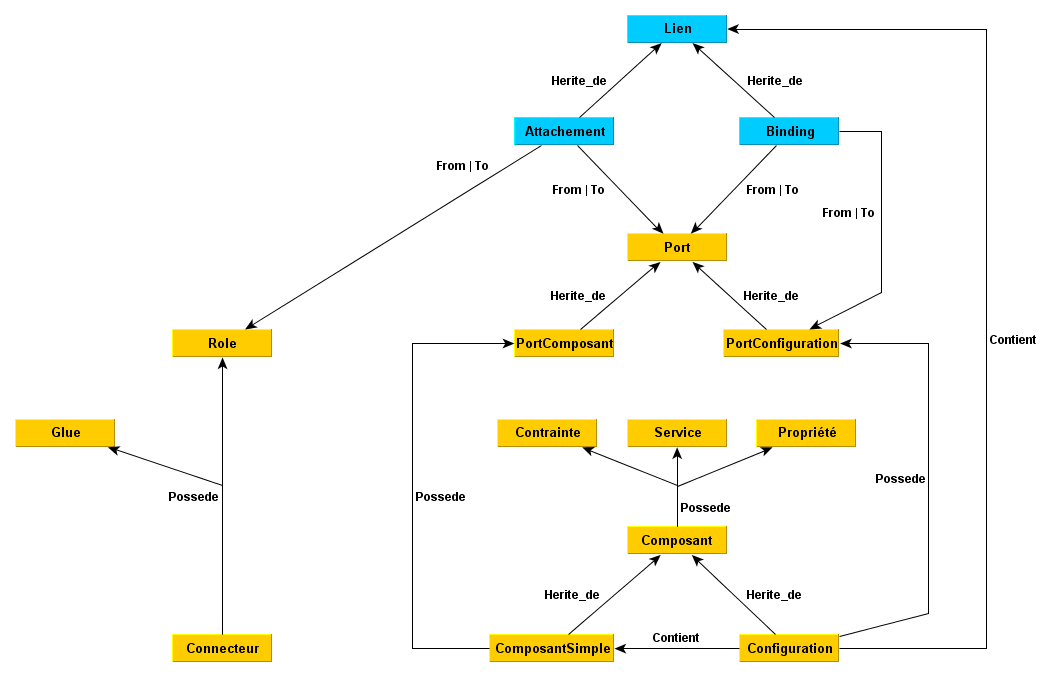
\includegraphics[scale=0.5]{../images/m2.PNG}
		\caption{représentation du M2}
	\end{figure}
		
\clearpage